\documentclass{article}
\usepackage{graphicx} % Requerido para insertar imagenes
\graphicspath{ {img/} }
\usepackage[square,numbers]{natbib}
\usepackage[spanish]{babel}
\usepackage{amsmath}
\usepackage{float}



\title{Tarea 5}
\author{Sonia Torres Ibarra}
\date{\today}


\begin{document}

\maketitle

\section{Introducción}

En el análisis de datos, los algoritmos no supervisados juegan un papel fundamental al permitir descubrir estructuras subyacentes sin necesidad de etiquetas o clases predefinidas. Estos métodos son ampliamente utilizados en contextos donde se busca identificar patrones, segmentar observaciones o reducir la complejidad de los datos, como en la exploración de clientes, análisis de comportamiento o clasificación automática de información.\\

Entre las técnicas más comunes se encuentran los algoritmos de clustering, que agrupan elementos con características similares. Sin embargo, la elección del algoritmo adecuado depende tanto de la naturaleza de los datos como de la forma en que se desea representar la similitud entre observaciones. En este trabajo se investigó una alternativa adicional a los métodos vistos en clase, considerando el modelo DBSCAN, el cual ofrece ventajas frente a algoritmos clásicos como k-means, especialmente cuando los datos presentan ruido, densidades variables o formas de agrupamiento no esféricas.\\

Asimismo, se abordan métricas de evaluación para determinar el número óptimo de grupos, tales como los índices de Silhouette Score y Davies-Bouldin, que permiten cuantificar la calidad de la segmentación obtenida. La combinación de estos enfoques busca no solo obtener una agrupación más representativa, sino también justificarla matemáticamente a partir de medidas objetivas de desempeño.\\

Finalmente, se presenta la aplicación práctica de un algoritmo no supervisado a un conjunto de datos reales, acompañada del análisis de resultados, la discusión de las métricas empleadas y la referencia a trabajos científicos previos relacionados con la metodología implementada.
\clearpage
\section{Descripción de los datos}

La Comisión Nacional Bancaria y de Valores (CNBV), en colaboración con el Instituto Nacional de Estadística y Geografía (INEGI), realizaron la Encuesta Nacional de Inclusión Financiera (ENIF) 2024. Su objetivo es generar información estadística e indicadores oficiales a nivel nacional que permitan a las autoridades financieras hacer diagnósticos, diseñar políticas públicas y establecer metas en materia de inclusión y educación financieras. Asimismo, incorporar cambios y actualizaciones para dar atención a nuevos requerimientos de información y consideraciones en la Política Nacional de Inclusión Financiera (PNIF).

\section{Antecedentes}

Investigaciones relacionadas:\\

El autor Cando \cite{candofacultad} menciona que "DBSCAN, se distingue por su capacidad para identificar agrupaciones de formas irregulares y destacar puntos de datos aislados como outliers, lo
que lo convierte en una herramienta valiosa para discernir comportamientos financieros
altamente atípicos entre los socios" .

\section{Metodología}
El DBSCAN es un algoritmo no supervisado muy conocido en materia de Clustering. Fue presentado en 1996 por Martin Ester, Hans-Peter Kriegel, Jörg Sander y Xiawei Xu.\cite{ml_dbscan_ds}\\

El DBSCAN es un algoritmo sencillo que define los clústeres mediante la estimación de la densidad local. Se puede dividir en 4 etapas:
\begin{itemize}
  \item Para cada observación miramos el número de puntos a una distancia máxima $\epsilon$ de ella. Esta zona se denomina $\epsilon$-vecindad de la observación.
  \item Si una observación tiene al menos un cierto número de vecinos, incluida ella misma, se considera una observación central. En este caso, se ha detectado una observación de alta densidad.
  \item Todas las observaciones en la vecindad de una observación central pertenecen al mismo clúster. Puede haber observaciones centrales cercanas entre sí. Por lo tanto, de un paso a otro, se obtiene una larga secuencia de observaciones centrales que constituyen un único clúster.
  \item Cualquier observación que no sea una observación central y que no tenga ninguna observación central en su vecindad se considera una anomalía.
\end{itemize}

DBSCAN por lo general utiliza la distancia euclidiana\\

\begin{math}
d(p,q)=\sqrt{(p_1-q_1)^2+(p_2-q_2)^2+...+(p_i-q_i)^2+...+(p_n-q_n)^2}=\sqrt{\sum_{i=1}^{n} (p_i-q_i)^2}
\end{math}\\

En cada observación, para contar el número de vecinos a como máximo una distancia $\epsilon$, calculamos la distancia euclidiana entre el vecino y la observación y comprobamos si es inferior a $\epsilon$.

DBSCAN utiliza dos parámetros principales \cite{datacamp}:
\begin{itemize}
    \item eps (épsilon): La distancia máxima entre dos puntos para que se consideren vecinos.
    \item min samples: El número mínimo de puntos necesarios para formar una región densa.
\end{itemize}

Por lo tanto, es necesario definir 2 datos antes de utilizar DBSCAN:
\begin{itemize}
\item ¿Qué distancia $\epsilon$ hay que determinar para cada observación la $\epsilon$-vecindad? 
\item ¿Cuál es el número mínimo de vecinos necesario para considerar una observación como una observación central?
\end{itemize}


En este trabajo, para seleccionar los parámetros óptimos del algoritmo DBSCAN , se utilizaron métricas internas de validación de clustering, específicamente el Silhouette Score y el Davies-Bouldin Index.\\

El Silhouette Score \cite{silhoutte} mide la cohesión interna de un cluster y la separación entre clusters. Para cada punto $i$ , se calcula la distancia promedio a los demás puntos de su propio cluster ($a_i$) y la distancia promedio al cluster más cercano ($b_i$), dando como resultado un valor:

\begin{math}
s_i=\frac{b_i-a_i}{max(a_i,b_i)} \
\end{math}\\

con rango [−1,1], donde valores cercanos a 1 indican clusters bien definidos y separados, valores cercanos a 0 indican puntos en los límites de los clusters, y valores negativos sugieren posible asignación incorrecta \cite{scikitlearn_clustering}.

El coeficiente de la Silhouette ($s_i$) se define para cada clúster. Cuando se dispone de más de dos clústeres se calcula el valor promedio de la Silhouette para disponer de una medida de la calidad de los clústeres.\\

Por otro lado, el Davies-Bouldin Index (DBI) \cite{Davies_Bouldinen} se basa en relacionar la dispersión dentro de los clústeres (intra-clúster) y la separación entre clústeres (inter-clúster). Por un lado, la dispersión intra-clúster mide la separación de los puntos dentro de cada clúster. Una dispersión intra-clúster baja indica que los puntos dentro de un grupo están muy cercanos entre sí, algo que es deseable en un buen clustering. Por otro lado, la dispersión inter-clúster mide la separación entre los grupos. Una dispersión inter-clúster alta indica que los grupos están muy alejados entre sí, lo que también es deseable en un buen clustering. El índice de Davies-Bouldin se construye como el cociente de ambos valores. Por lo que cuando los clústeres están separados y son compactos el valor de este índice se minimiza.:


\begin{math}
DB=\frac{1}{k} \sum_{i=1}^{k} \max_{j \neq i} \frac{S_i+S_j}{M_{ij}} \\
\end{math}

donde $S_i$ es la dispersión promedio dentro del cluster $i$ y $M_{ij}$ la distancia entre los centroides de los clusters $i$ y $j$. Valores bajos de DBI indican clusters más compactos y mejor separados.

Para aplicar estas métricas, se probó DBSCAN con distintas combinaciones de eps y min samples, calculando Silhouette y Davies-Bouldin para los clusters detectados (excluyendo outliers). La combinación que maximizó el Silhouette Score y minimizó el Davies-Bouldin Index fue seleccionada como óptima, asegurando así una segmentación más representativa y coherente de los datos.

\section{Resultados}

En la figura 1 (p.\pageref{fig:resultado}) se muestran los resultados de aplicar DBSCAN sobre los datos, evaluando distintos valores de los parámetros eps y min samples. Se incluyeron métricas de validación  como Silhouette Score y Davies-Bouldin Index para determinar la calidad de los clusters obtenidos y los parámetros a utilizar.

\begin{figure}[H]
    \centering
    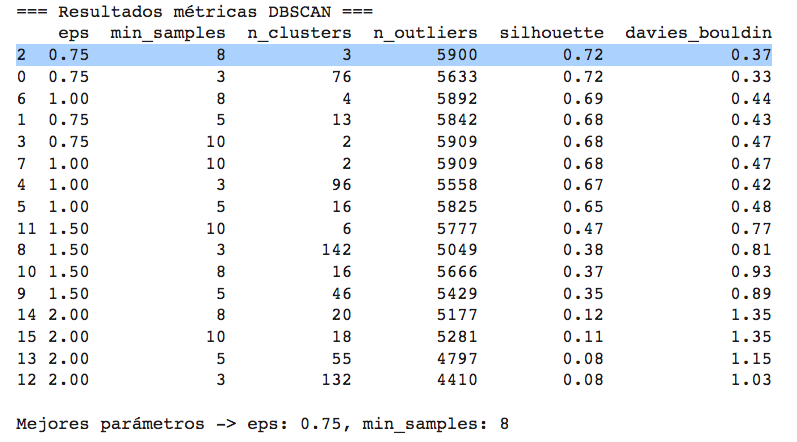
\includegraphics[width=1\linewidth]{Resultado_1.png}
    \caption{Resultados para pruebas DBI y Silhouette}
    \label{fig:resultado}
\end{figure}

El valor más alto de Silhouette (0.72) se obtiene para eps=0.75 y min samples=3 o min samples=8. Esto sugiere que los clusters detectados bajo estos parámetros presentan una buena separación relativa entre ellos.\\

Para el índice de Davies-Bouldin, los valores más bajos (0.33–0.37) se observan también en los parámetros de eps=0.75 y min samples bajos, corroborando la cohesión detectada por Silhouette.\\

Considerando ambas métricas, los parámetros eps=0.75 y min samples=8 fueron seleccionados como los más adecuados, ya que logran un balance entre número razonable de clusters y alta calidad de agrupamiento.\\

DBSCAN, con eps=0.75 y min samples=8, detecta tres grupos principales de usuarios y destaca la heterogeneidad mediante la gran cantidad de outliers.

\begin{figure}[H]
    \centering
    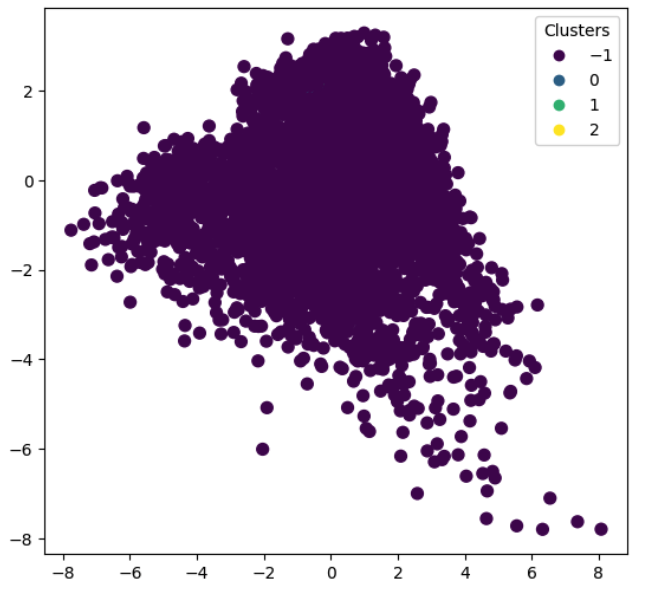
\includegraphics[width=0.5\linewidth]{Resultado_2.png}
    \caption{Gráfico DBSCAN con los parámetros seleccionados.}
    \label{fig:dbscan:graphic}
\end{figure}


\begin{table}
\caption{Clusters obtenidos}
\centering
\begin{tabular}{|l|r|} \hline 
Cluster & Casos \\ \hline \hline
-1      & 5900  \\ \hline
0       & 20   \\ \hline
1       & 15  \\ \hline
2       & 9    \\ \hline
\end{tabular}
\label{tab:clusters}
\end{table}

\section{Conclusiones y discusión}

Esta tarea permitió explorar la aplicación del algoritmo DBSCAN, como una alternativa para la detección de patrones y agrupamientos en aprendizaje no supervisado. A diferencia de otros métodos más rígidos como k-means, DBSCAN no requiere definir previamente el número de grupos.

Para mejorar la calidad del agrupamiento y reducir el uso de recursos computacionales, se aplicó una reducción de variables mediante PCA (Análisis de Componentes Principales), que no se menciono en los resultados ya que no era parte del fin de esta actividad. Posteriormente, se realizó una búsqueda de los parámetros eps y min samples.

La búsqueda de parámetros se realizo con el índice de Silhouette y el índice de Davies-Bouldin. Estos cálculos permitieron analizar la relación interna de los clústeres y la separación entre ellos, proporcionando una visión más completa del desempeño del modelo. Los valores reflejaron una estructura de clústeres bien definida y con baja superposición entre grupos. Sin embargo, se identificó una cantidad considerable de outliers, lo que sugiere la existencia de observaciones atípicas o de baja densidad en el conjunto de datos.

Los hallazgos confirman que DBSCAN es un buen algoritmo para la identificación de patrones en datos complejos, siempre que se realice una selección cuidadosa de sus parámetros y se complementen los resultados con métricas de validación adecuadas. 

\bibliographystyle{abbrvnat}
\bibliography{biblio}


\end{document}








